\documentclass[12pt,a4paper]{article}
\usepackage[T2A]{fontenc}
\usepackage[utf8]{inputenc}
\usepackage[russian]{babel}
\usepackage{graphicx}
\usepackage{booktabs}
\usepackage{hyperref}
\usepackage{geometry}
\geometry{margin=2.5cm}

\title{Отчёт о производительности\\Image Quality Sorter}
\author{Student}
\date{2026}

\begin{document}
\maketitle

\section{Цель}

Проект сортирует изображения по резкости. Основная метрика --- variance of
Laplacian: изображение переводится в оттенки серого, затем сворачивается с
дискретным оператором Лапласа, после чего считается дисперсия результата. Чем
больше значение, тем больше сильных локальных перепадов яркости и тем выше
оценка резкости.

\section{Данные}

Для проверки производительности используются синтетические изображения с
шахматной высокочастотной структурой. Такой набор удобен для воспроизводимого
эксперимента: генератор не зависит от внешних файлов и создаёт одинаковые
данные при каждом запуске. Размеры изображений: $128^2$, $256^2$, $512^2$,
$1024^2$ и $2048^2$ пикселей.

\section{Методика измерения}

Скрипт \texttt{report/generate\_figures.py} для каждого размера создаёт массив
\texttt{float64}, вычисляет Laplacian variance несколько раз и берёт медиану
времени. Медиана выбрана вместо среднего, чтобы уменьшить влияние случайных
скачков времени выполнения.

\section{Результаты}

\begin{figure}[h]
  \centering
  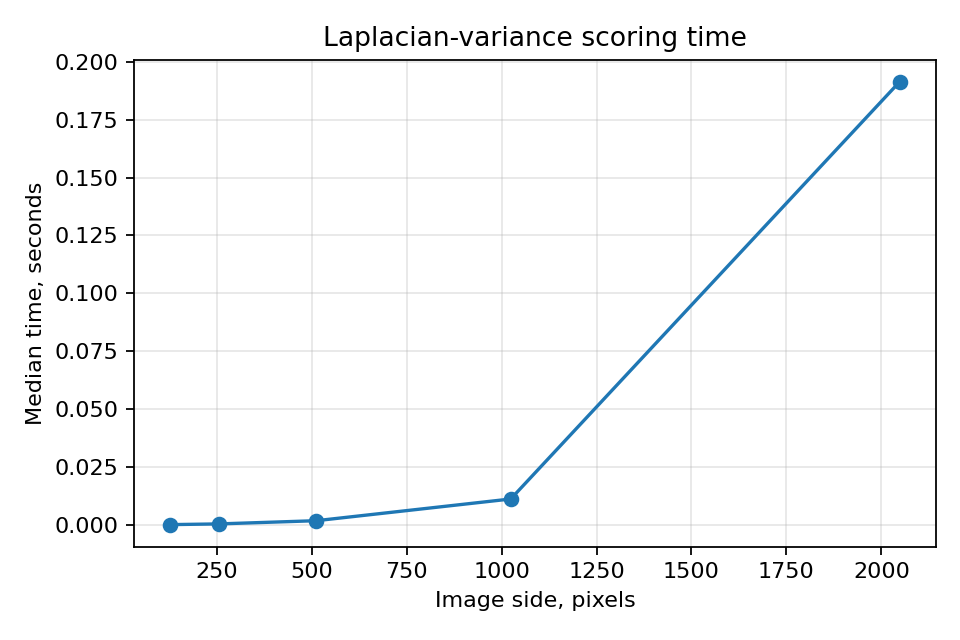
\includegraphics[width=0.85\textwidth]{figures/performance.png}
  \caption{Время вычисления variance of Laplacian для синтетических изображений.}
\end{figure}

\begin{table}[h]
  \centering
  \begin{tabular}{ll}
    \toprule
    Параметр & Значение \\
    \midrule
    Основная операция & дискретная свёртка $3 \times 3$ без OpenCV \\
    Тип массива & \texttt{numpy.float64} \\
    Повторы на размер & 7 \\
    Агрегация & медиана \\
    \bottomrule
  \end{tabular}
  \caption{Параметры эксперимента.}
\end{table}

\section{Вывод}

Сложность алгоритма линейна по числу пикселей: каждый пиксель участвует в
фиксированном числе арифметических операций. Поэтому при увеличении стороны
изображения в два раза время растёт примерно в четыре раза. Для CLI это
означает, что основное узкое место на больших наборах данных --- количество
пикселей и скорость чтения изображений с диска, а не сортировка результатов.

\end{document}
